% CVPR 2022 Paper Template
% based on the CVPR template provided by Ming-Ming Cheng (https://github.com/MCG-NKU/CVPR_Template)
% modified and extended by Stefan Roth (stefan.roth@NOSPAMtu-darmstadt.de)

\documentclass[10pt,twocolumn,letterpaper]{article}

%%%%%%%%% PAPER TYPE  - PLEASE UPDATE FOR FINAL VERSION
%\usepackage[review]{cvpr}      % To produce the REVIEW version
%\usepackage{cvpr}              % To produce the CAMERA-READY version
\usepackage[pagenumbers]{cvpr} % To force page numbers, e.g. for an arXiv version

% Include other packages here, before hyperref.
\usepackage{graphicx}
\usepackage{amsmath}
\usepackage{amssymb}
\usepackage{booktabs}


% It is strongly recommended to use hyperref, especially for the review version.
% hyperref with option pagebackref eases the reviewers' job.
% Please disable hyperref *only* if you encounter grave issues, e.g. with the
% file validation for the camera-ready version.
%
% If you comment hyperref and then uncomment it, you should delete
% ReviewTempalte.aux before re-running LaTeX.
% (Or just hit 'q' on the first LaTeX run, let it finish, and you
%  should be clear).
\usepackage[pagebackref,breaklinks,colorlinks]{hyperref}


% Support for easy cross-referencing
\usepackage[capitalize]{cleveref}
\crefname{section}{Sec.}{Secs.}
\Crefname{section}{Section}{Sections}
\Crefname{table}{Table}{Tables}
\crefname{table}{Tab.}{Tabs.}


%%%%%%%%% PAPER ID  - PLEASE UPDATE
\def\cvprPaperID{*****} % *** Enter the CVPR Paper ID here
\def\confName{CVPR}
\def\confYear{2022}


\begin{document}

%%%%%%%%% TITLE - PLEASE UPDATE
\title{ALTEGRAD 2024 - Data Challenge Report\\ CGM Team}

\author{Channdeth Sok\\
Institution ?\\
{\tt\small e-mail ? }
% For a paper whose authors are all at the same institution,
% omit the following lines up until the closing ``}''.
% Additional authors and addresses can be added with ``\and'',
% just like the second author.
% To save space, use either the email address or home page, not both
\and
Gleb Goncharov\\
M2DS\\
{\tt\small e-mail ?}
\and
Marceau Leclerc\\
M2DS\\
{\tt\small marceau.leclerc@outlook.fr}
}
\maketitle

%%%%%%%%% ABSTRACT
\begin{abstract}
   This report is part of the work our team produced in the framework of the ALTEGRAD 2024 Data Challenge. We will present most of our experiments that ended up being interesting, either because their implementation was insightful in some way or because the results they gave at the task at hand are interesting to report. Our goal in this document is to explain our reasoning and how we advanced through this project.
\end{abstract}

%%%%%%%%% BODY TEXT
\section{Introduction}
\label{sec:intro}
The task we aim to tackle is a down-scaled version of the one presented in \cite{evdaimon2024neuralgraphgeneratorfeatureconditioned}, to which end was introduced the architecture of the Neural Graph Generator (NGG). The goal is to generate graphs presenting the key features (e.g. the number of nodes, average degree, etc.) prompted by the user. In the code we were provided, these features indeed were given in a prompt format and were exactly 7, unlike in \cite{evdaimon2024neuralgraphgeneratorfeatureconditioned} where there are up to 15 features. To accomplish this, our baseline was NGG, an architecture that combines a variational autoencoder (VAE) that can be trained to reconstruct graphs while producing a latent space in the bottleneck, and a diffusion model (DM) which can be trained to sample realistic latent space vectors using the conditioning, i.e. the features we want to recover.
\medskip \newline

In this report we will present the data we were handed and how we came to use it like we did, as well as our evaluation metrics. From there we will go through the different models, tweaks and strategies we used to try and better accomplish the task, as well as report their respective performances. Finally we will discuss our results and the lessons they yielded.

%%%%%%%%%%%%%%
\section{Related Work}
\label{sec:related_work}
We will here briefly present the sources of our inspirations when navigating this project. We already introduced the framework of NGG \cite{evdaimon2024neuralgraphgeneratorfeatureconditioned}.

\noindent
\textbf{Contrastive Learning}. To try and improve upon NGG, we experimented with a contrastive training objective. CLIP \cite{CLIP} was introduced to align visual and textual spaces with great success. Following it, GraphCLIP \cite{graphCLIP} was introduced to align the "graph modality" with the textual one. We decided to base our contrastive experiments on this philosophy, adapting the method to our (less complex) task where it was relevant, i.e. when training NGG's VAE.

\medskip
\noindent
\textbf{Language Models}. The data features provided were in the forms of prompts, it then seemed natural to try and encode this language data using LLMs, specifically trying BERT \cite{bert} that has proven to produce sentence embeddings of high quality. Still on the topics of LLMs, we had the idea of directly using a finetuned LLM to directly predict the graphs' edgelists out of the prompts. To operate such finetuning in practice with hardware available to us, we chose to train a LoRA \cite{lora} for the memory-efficiency of this method. 

\noindent
\textbf{Graph embedding}. We experimented with a different method of graph embedding than the one (spectral) provided. Deepwalk \cite{deepwalk} is a method that embeds graphs by running a fixed number of fixed-length random walks on all the nodes. This per-node representation is then mapped to a learned embedding space using a method such as \cite{word2vec}. 

\section{Approach and results}
\label{sec:approach_results}
We make the choice of presenting the methods we used along their results. In our opinion, this clarifies our exploratory approach and helps to better make sense of the path we followed. To that end we will start by introducing the metric we came up with to evaluate our progress and models, and then go through our experiments in a somewhat chronological fashion.

\subsection{Evaluation metric}
\label{subsec:eval}
We will further discuss the original training metrics when elaborating on NGG in Section \ref{subsec:NGG}. To enable us to compare our models without completely relying on kaggle submissions, we came up with an evaluation script that can score a sequence of graph edglelists (following the structure of the target output to submit). To that end we simply took the description of the evaluation in the provided instruction sheet. The submissions were described as being scored according to a mean average error (MAE) directly on the features of the output graphs, compared to the desired features inputted. We simply reproduced that with the obvious {\tt NetworkX} Python library utilitaries. The only choice we made was regarding the number of communities feature, for which the computing algorithm incorporates stochasticity. To try and circumvent the noise induced as a consequence without adding too much computing time, we ran 10 Louvain community computations and averaged their outputs. We also reversed-engineered the fact that the features were standard-scaled in order not to bias the score towards the features that inherently have high numerical values, \eg the number of triangles or number of edges.

\noindent
The method described above was implemented in a python script we could run either on demand or at the end of a training procedure when generating the output graph. It was not used as a validation metric inside a training procedure. We abused of the test set in that way, even though it is the opposite of rigorous practice. We motivate that choice by the fact that this project is part of a kaggle competition, and we did want to score as high as possible. This evaluation script was somewhat reliable, in particular of high MAE values, but did lack precision when obtaining better scores, all in all limiting our ability to mindlessly overfit using it. XXX TODO (maybe) : graph of the kaggle score vs evaluation script.
\noindent
We did notice at late stage of the project that a very similar metric was handed in the github associated to \cite{evdaimon2024neuralgraphgeneratorfeatureconditioned}. We did not use it at all and entirely complied with the "no external code" rule of the project.

\subsection{Handed data}
\label{subsec:data}
The data provided was formatted as follows. We had a given prompt that described the graph to predict's expected features. These were the number of nodes, edges, average degree, number of triangles, global clustering coefficient, maximu k-core and number of communities. These 7 features were always present and always in this exact order. Apart for the test set, these prompts were paired with corresponding graphs. The volume of data was as so:
\begin{itemize}
    \item A training set comprising 8000 description-graph pairs.
    \item A validation set comprising 1000 description-graph pairs.
    \item A test set comprising 1000 descriptions, the graphs having to be predicted and being the object of the comptetion scoring.
\end{itemize}

When running our custom experiments (from Section \ref{subsec:bert}, we chose to standard-scale the features in order to ensure consistency in our approach.

\subsection{NGG baseline}
\label{subsec:NGG}
The handed NGG \cite{evdaimon2024neuralgraphgeneratorfeatureconditioned} architecture is comprised of a VAE that encodes a graph's embedding to a latent space, and decodes the latent representation to graph adjacency matrix, that aims to recover a graph with corresponding features. To make use of this latent space, a DM denoises a standard vector conditionally to the features after these are embedded via a simple MLP. The exact architecture goes as so:

\begin{itemize}
    \item The encoder maps an embedding of size 10 to a latent representation of dimension 32 through 2 layers of hidden dimension 64.
    \item The decoder maps the latent representation to the adjacency matrix through 3 layers of hidden dimension 256.
    \item The DM uses 500 timesteps to map a normal vector of dimension 32 to a plausible latent representation through 3 layers of dimension 512 to which are concatenated the features' embeddings.
    \item These features embedding are obtained via an MLP that maps the 7 features vector to a vector of size 128 through 2 layers of dimension 128.
\end{itemize}

The general base training workflow goes as follows:
\begin{itemize}
    \item The features are directly extracted using the consistent prompt format.
    \item The graphs go through a spectral embedding to retrieve the 10 most important spectral features.
    \item The VAE is trained first using two objectives:
    \begin{itemize}
        \item A reconstruction objective on the decoded adjacency matrix.
        \item A transport objective in the form of the minimization of a Kullback-Leibler divergence in the latent space.
    \end{itemize}
    These losses are summed with a weighting of 0.05 to the KLD loss to define the VAE's loss.
    \item The DM and feature MLP are then trained simultaneously to recover the associated latent representation using a simple L1 loss.
    \item The then trained model can be used to sample a latent representation of the requested features that is then decoded to predict an associated graph's adjacency matrix, that can be used to recover an edgelist.
    
\end{itemize}
This original model typically produces  - after 200 and 100 epochs for the VAE and DM respectively and no early stopping procedure, which is enough for the models' losses to converge on the validation set - outputs that score an MAE of around \textbf{0.88621}, translating to a score of around \textbf{}{0.89554} with our evaluation metric. This was our provided baseline.

\subsection{Style transfer approach baseline}
\label{subsec:KNN}
@Gleb if you don't mind. (KNN).

\subsection{Graph embedding with Deepwalk}
\label{subsec:deepwalk}
We wanted to experiment with a different embedding than the spectral one to see if it would improve the latent representation. To that end we used the Deepwalk \cite{deepwalk} method. To find a good compromise between a fine representation and a fast obtention, we chose to run 10 walks of size 12 per node. The generated embeddings were set to be of dimension 10, in order to fairly compare them with the spectral embeddings. From there we could run the base NGG workflow described in \ref{subsec:NGG} that yielded an MAE (ours) of \textbf{0.89538}. As this was not a significant improvement, we chose to stick with a spectral embedding of the graphs for the rest of the project.

\subsection{Prompt embedding}
\label{subsec:bert}
Similarly, we wanted to try embedding the features in a more complex space than the base 7-dimension representation. To that end we tried directly embedding the prompts with BERT \cite{bert} using a simple summing aggregation to get a 768-dimensional representation. This led to an a MAE (ours) of \textbf{0.89470}. To try and better it, we also concatenated this vector with the 7 features themselves, leading to score similar to the ones without any prompt embedding. As a consequence, we did not chose to embed the prompts in that way and kept going with the 7 features only.

\subsection{Base NGG tuning and data synthesis}
\label{subsec:data_gen}
We did try varying the depths and widths of the various bricks of NGG to try and see if we could improve the MAE. These experiments were unfruitful. It does seem indeed that the default hyperparameters of the handed NGG model were close the optimal one for the base set up (including parameters and datasets). However we did get a somewhat significant improvement when generating new data.
\textbf{Data synthesis}. We did want to generate more data from the get go in order to see if it would allow NGG to learn further, as well as to have them for the other architectures we would try. Upon exploring the data and reading \cite{evdaimon2024neuralgraphgeneratorfeatureconditioned} in details we figured it wouldn't be efficient to simply reverse engineer the exact synthesis process, there being more than 15 graph generation algorithms. To circumvent that difficulty, we chose to simply slightly modify the graphs in the original training and validation sets. For each graph $G$ in those sets, we chose to generate 6 new graphs as follows. Define $m$ to be an integer sampled uniformly at random between 1 and $\lfloor 0.20 * n \rfloor$ where $n$ is the number of nodes in $G$.
\begin{itemize}
    \item 2 were generated using $G's$ adjacency matrix $A$ by simply "flipping" values at random, \eg a 0 would become a 1 and conversely. This was of course done in a symmetric way $m$ times.
    \item 2 were generated deleting $m$ nodes in $G$, and their corresponding edges.
    \item 2 were generating adding $m$ nodes in $G$, and connecting them uniformly at random to $p$ other existing nodes in $G$, sampling $p$ as the degree of an existing node in $G$ selected uniformly at random as well. This way, added nodes are connected to other nodes in a way that isn't dramatically different as the other existing nodes.
\end{itemize}
After these graphs were generated, we could pair them with their prompts by simply computing their 7 features of interest and placing them in one of the 2 prompt templates that were present in the original dataset.

Running NGG on this enhanced dataset (the combination of both the original dataset and the generated one) led us to our first noticeable improvement, yielding a MAEs of \textbf{0.84613} (kaggle) and \textbf{0.86101} (our script). We still needed to make drastic changes to better these scores.

\subsection{Finetuning LLMs}
\label{subsec:LLMs}
An exotic idea that seemed relevant for us to give it a chance was to just finetune (using a LoRA \cite{lora}) a language model to directly spit out a graph's edgelist from a prompt. To that end a first attempt was done in the following setting. First we generated short very standard prompts (in order not to waste context on it) as well as the expected output in the form of the corresponding graph's edgelist. A LoRA of rank 16 was trained along Microsoft's Phi3 Mini Instruct quantized in 4 bits. This allowed training of said adapter on a single 8GB laptop GPU with batch sizes of 1. We chose for this attempt to sacrifice all the efficiency we could to maximize the yielding model's potential. 

\noindent
Training was run in under 8 hours. However the results were very disappointing. We did not expect them to be perfect - as this version of Phi3 had a maximum context length of 4096 tokens, which was not enough to cover our prompt-answer pairs that could go up to 6000 tokens for the most heavily connected graphs. But in fact this attempt yielded nonsensical results that did not comply with the template we trained it on.

@Channdeth can you insert what you did here ?


\subsection{Conditioning NGG's VAE}
\label{subsec:conditioning}
From this subeection onwards, all training procedures incorporate an early stopping criterium.
@Gleb if you have the time to, otherwise I'll do it sometime next week.
Insert CondVAE figure however possible here.
I will adapt the next subsection depending on the scores and what you fill in here (if you put the scores with and/or without denoiser).


\subsection{Ablation of the denoiser}
\label{subsec:ablation_denosier}
The previous experiments were enhanced when removing the denoiser. TODO (marceau), not forgetting the table with all the results that clearly prove the denoiser can't do better than pure noise. Start by saying we observed that the mlp in the denoiser was useless.

\subsection{Contrastive learning objective in NGG}
\label{subsec:CLIP}
Independently from the previous subsection \ref{subsec:conditioning}, we tried improving NGG's latent space by incorporating a contrastive objective instead of the KLD loss. Inspiring ourselves from \cite{CLIP} and \cite{graphCLIP}, we chose to try and make the graph encoder (the GIN) in NGG learn a latent space that minimizes the contrastive loss $\mathcal{L_\text{c}}$ defined below. To that end, we left the VAE untouched but incorporated an MLP to embed the features of a given graph $G$. A sketch of the workflow is provided in Fig. \ref{fig:CLIP}.

\begin{figure}[h]
    \centering
    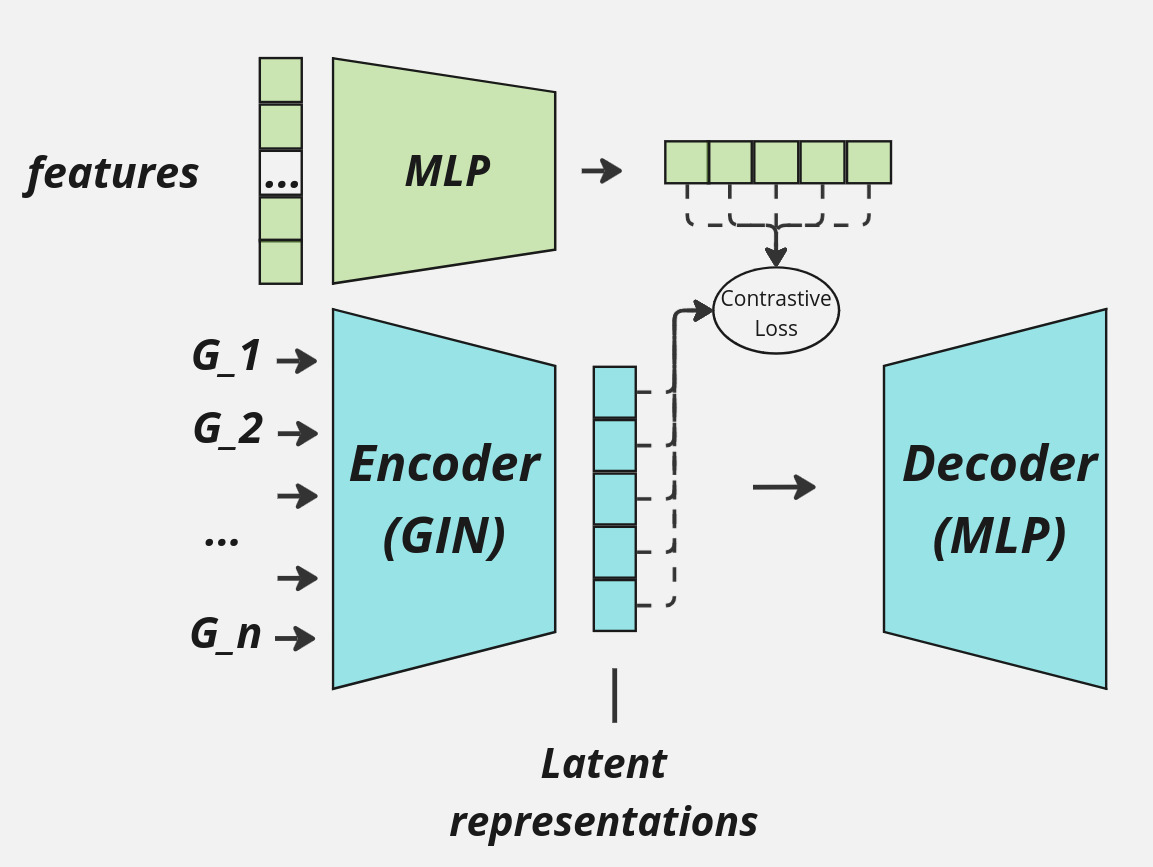
\includegraphics[width=.8\linewidth]{figures/CLIP.jpg}
    \caption{Addition of a feature MLP to get a contrastive loss.}
    \label{fig:CLIP}
\end{figure}

\noindent
\textbf{Contrastive loss}. Given a batch of $n$ graphs $\{G_1, ..., G_n\}$ and its label vector $l = \{1, ..., n\}$ :
\begin{enumerate}
    \item Embed the graph and feature batches in their respective encoders to get their representations $E_G$ and $E_f$ of sizes $n \times d_{\text{latent}}$ and $n \times d_{\text{feat}}$ (resp.).
    \item Compute $S = \frac{1}{T}(E_G \dot E_f$)the similarity matrix of size $n \times n$. Here $T$ is a temperature parameter fixed at 0.07.
    \item Compute the loss, CE denoting the cross-entropy function:\begin{equation}
    \mathcal{L_\text{c}} = \frac{1}{2}(\text{CE}(S, l) + \text{CE}(S^{T}, l))
\end{equation}
\end{enumerate}

\noindent
Now we can train this CLIP-ized NGG in two different ways.
\begin{itemize}
    \item We can either do it sequentially, first minimizing this contrastive loss and training both encoders, leaving the decoder untouched, before then freezing the graph encoder to produce latent representations from which we can train the decoder minimizing the original reconstruction loss. The upside of such sequential training is that we do indeed force the latent space to encode in some way information about the features, from which the decoder can then learn to reconstruct.
    \item The alternative way is to train this modified NGG "jointly", meaning that all the bricks are trained at once minimizing a loss that is the sum of the reconstruction and contrastive losses. For the presented results below we don't weigh these losses and add them as is. A few explorations showed adding a weighting only impacted the first training steps. The upside of this so called joint training is that the decoder can prevent the latent space from being too particular about the contrastive task.
\end{itemize} 

The results in Table \ref{tab:clip} were obtained using batches of size 1024 for the whole chain when learning jointly and 1024 for the contrastive task while 256 for the reconstruction task in the sequential workflow. In both cases, the original dataset enriched with the synthetic one was used, at yielded slightly better results in the case of the simple NGG. The denoiser was trained afterwards and used to sample new data.

\begin{table}[h!]
    \centering
    \begin{tabular}{|l|c|c|}
    
        \hline
        \textbf{Learning Procedure} & \textbf{MAE (Ours)} & \textbf{MAE (Kaggle)} \\
        \hline
        Sequential & 0.79587 & 0.80624 \\
        Joint & 0.80754 & 0.79519 \\
        \hline
    \end{tabular}
    \caption{MAEs of NGG integrating the contrastive procedures}
    \label{tab:clip}
\end{table}

Both workflows ended up yielding similar results. These were a slight improvement from the base NGG, but did not perform nearly as well as the conditional VAE presented in the previous subsection \ref{subsec:conditioning}. It then seemed natural to try and merge this contrastive learning task with the conditioned architecture, presented in the next subsection \ref{subsec:CLIP_cond}.

\noindent
Small remark, we did try to further use and freeze the contrastively learnt feature encoder in the denoiser instead of having it train its own MLP. A few runs showed it did not improve it, confirming further the results in subsection \ref{subsec:ablation_denosier}.
% using the featur encoder as feature mlp in the denosier



\subsection{Contrastive learning and conditionning of NGG}
\label{subsec:CLIP_cond}

\section{Tuning of the conditional VAE}
\label{sec:setup}
TODO : I might merge it with the cond vae subsection

The conditional VAE and random sampling in the latent space being our best result so far, it seemed natural to tune its architecture and see what we could squeeze out of it. We proceeded in the following way : we picked a hyperparameter \eg the hidden size of the decoder's layers, found the best one (using each time an early stopping criterium), and moved on to another hyperparameter, and so on and so forth. The best architecture is presented in Table \ref{tab:condvae_arch}. We also reported another very interesting result that we will make sense of.

\begin{table}[h!]
    \centering
    \small  % Small font for compactness
    \renewcommand{\arraystretch}{1.2}  % Increases row height slightly for readability
    \begin{tabular}{|l|c|c|}  % Vertical lines for all columns
        \hline
        \textbf{Hyperparameter} & \textbf{Best CondVAE} & \textbf{Small Latent Dim} \\
        \hline
        Encoder hid dim & 32 & 32 \\
        Decoder hid dim & 768 & 768 \\
        Conditioning hid dim & 48 & 48 \\
        Latent dim & 64 & 2 \\
        \# layers encoder & 4 & 4 \\
        \# layers decoder & 4 & 4 \\
        \hline
        MAE (ours) & 0.21641 & 0.24495 \\
        \hline
    \end{tabular}
    \caption{Conditional VAE architecture tuning}
    \label{tab:condvae_arch}
\end{table}

One thing that has to be noted is that if this "best" architecture produced the smallest MAE, it is likely due to luck. Indeed when trying out architectures in a "grid search" fashion, the MAE wouldn't vary much, only improved when increasing the hidden size of the feature MLPs and that of the decoder, suggesting these two bricks were solely responsible for the score being better. This was confirmed when setting the latent dimension to the ridiculously low value of 2 and obtaining a result that was still competitive. Note that when our MAE was of values between 0.22 and 0.25, the kaggle MAE was around 0.12 to 0.14.

\indent
The lesson from this tuning was rather clear : the features alone may enable us to predict good enough graphs.

\subsection{Total ablation and use of MLPs}
\label{subsec:mlps}

\subsection{Metric abuse}
\label{subsec:abuse}

\section{Experimental setup}
\label{sec:setup}



%%%%%%%%% REFERENCES
{\small
\bibliographystyle{ieee_fullname}
\bibliography{egbib}
}

\end{document}
